\documentclass{scrartcl}
\usepackage{etoolbox}
\usepackage{bbm}
\usepackage{amsmath}
\usepackage{mathabx}
\usepackage{graphicx}
\usepackage{float}
\usepackage{parskip}
\usepackage{indentfirst}
%\usepackage{subfigure}
\usepackage{subfig}
\usepackage{fancyhdr}
\pagestyle{fancy}
\setlength{\parskip}{0em}
\setlength{\parindent}{2em}

%-----------------------------------------------------------------------------
\begin{document}

%-----------------------------------------------------------------------------
% header
\lhead{Huwenbo Shi (603-778-363) shihuwenbo@ucla.edu}

% title
\newcommand*{\TitleFont}{
      \usefont{\encodingdefault}{\rmdefault}{b}{n}
      \fontsize{16}{20}
      \selectfont}
\newcommand*{\AuthorFont}{
      \usefont{\encodingdefault}{\rmdefault}{r}{n}
      \fontsize{12}{20}
      \selectfont}
\title{\TitleFont SoCal: supervised genotype calling via ellipsoidal
separation for Affymetrix SNP microarray}
\author{\AuthorFont Huwenbo Shi (603-778-363) shihuwenbo@ucla.edu}
\date{}
\maketitle
%-----------------------------------------------------------------------------










%-----------------------------------------------------------------------------
% introduction
\section{Introduction}

\par
% background
% need to add why genotype calling is important
SNP microarray is a cost--effective approach to genotype samples for specific
association studies. % cite
In Affymetrix SNP microarrays, oligonucleotide probes are first used to bind
DNA fragments containing SNPs. % cite
Then, for each SNP, a fluorescence scanner quantifies perfect match (PM) and
mismatch (MM) for each of the two alleles, denoted by A and B, on
each strand of the DNA fragment. %cite
The genotype calling procedure for SNP microarray consists of two steps.
In the first step, information from microarray is summarized to obtain the
intensities, $\theta_A$ and $\theta_B$, of the two alleles of each SNP.
In the second step, SNPs are classified into genotype AA, AB, or BB based on
the allele intensities they generate.
The focus of this article is on the second step of the genotype calling
procedure---genotype classification using summarized allele intensities.

\par
% specific background
For a specific SNP, if a sample has genotype AA or BB, the intensity,
$\theta_A$ or $\theta_B$, will be higher respectively. 
If a sample has genotype AB, the intensities, $\theta_A$ and $\theta_B$,
will be similar.
If one plots $log(\theta_A)$ versus $log(\theta_B)$ of a SNP for a number of
samples, normally 3 ellipsoidal clusters are observed, one for each genotype,
as shown in Figure~\ref{fig:intro_genclus}.
Many genotype calling algorithms use model--based unsupervised clustering
methods to identify clusters and then assign genotypes to each cluster.
To estimate model parameters, these methods use the EM algorithm, which is
sensitive to starting parameters and slow to converge.
Rabbee et al. proposed the RLMM algorithm, a supervised genotype calling
method that uses reference genotype calls to form Gaussian decision
boundaries for each genotype.
This method involves fitting a linear mixed model, which can be computationally
intensive.

\par
% problem
As the number of probes on SNP microarrays and the number of individuals involved
in association studies continue to increase, both fast and accurate genotype
calling algorithms are needed.

% intro genotype cluster figure
\begin{figure}[H]
\centering
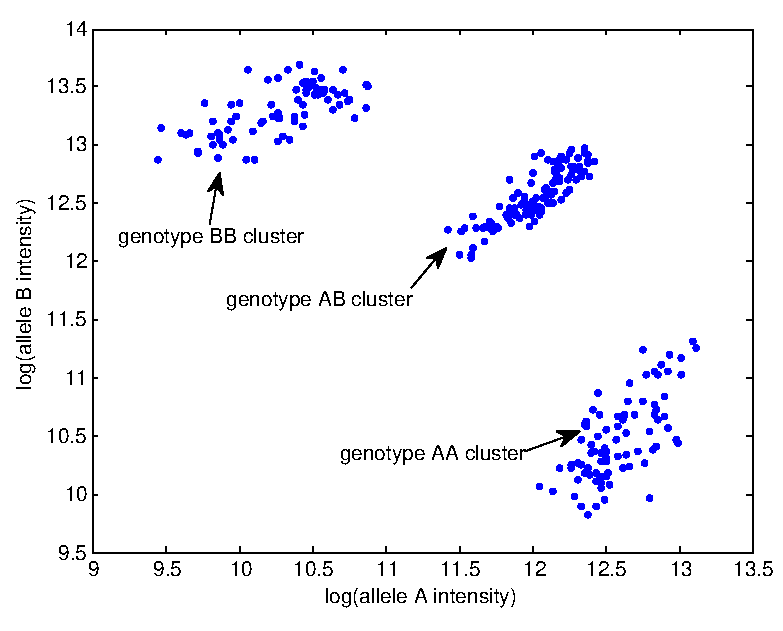
\includegraphics[scale=0.75]{intro_figs/intro_genotype_clusters.pdf}
\caption{Genotype clusters obtained from Affymetrix SNP array
allele intensity values}
\label{fig:intro_genclus}
\end{figure}

%-----------------------------------------------------------------------------










%-----------------------------------------------------------------------------
% method
\section{Method}

% overview of method
\subsection{Overview of SoCal's genotype calling procedure}

\par
SNP allele intensities are first summarized from raw microarray data using
SNPRMA, which removes non-biological effect from the data.
After this step, SoCal calls genotypes in two steps.
In the first step, SoCal finds ellipsoidal regions containing each of the
genotype of a SNP using reference genotype calls.
In the second step, SoCal classifies samples with unknown genotypes using
minimum distance classification.

% pattern separation via ellipsoids
\subsection{Pattern separation by ellipsoid}

\par
An ellipsoid $\mathcal{E} \subseteq \mathbbm{R}^{n}$ can be expressed as
$\mathcal{E} = \{x \in \mathbbm{R}^{n} | (x-c)^TE(x-c)\leqslant1\}$, where
$c$ is the center of the ellipsoid, and $E$ a positive definite matrix
denoting the shape and orientation of the ellipsoid.
Let $\{a_i\}$ be the points to be included in an ellipsoid, and $\{b_j\}$
be the points to be excluded, the problem of ellipsoidal separation is to find
$c$ and $E$ such that $(a_i-c)^TE(a_i-c)\leqslant1 \, \forall i$ and
$(b_j-c)^TE(b_j-c)>1 \, \forall j$.

% ellipsoidal pattern separation formulation
\subsection{Forming ellipsoidal decision regions for each genotype}

\par
Let $G=\{AA,AB,BB\}$ be the set of genotypes of a SNP, and $J_{AA}$, $J_{AB}$,
$J_{BB}$ the index set of samples with the corresponding genotype.
Let $X=\{(log(\theta_A),log(\theta_B))_i|i=1,\cdots,
|J_{AA}|+|J_{AB}|+|J_{BB}|\}$ be the set of log transformed allele intensities
of all the samples, and $X_{AA}=\{x_j|x_j \in X, j \in J_{AA}\}$,
$X_{AB}=\{x_j|x_j \in X, j \in J_{AB}\}$,
$X_{BB}=\{x_j|x_j \in X, j \in J_{BB}\}$ the set of log transformed allele
intensities from samples having the corresponding genotype.

\par
To find the ellipsoid that includes $X_{AA}$ and excludes
$X_{AB} \cup X_{BB}$, one
sets $\{a_i\}=X_{AA}$ and $\{b_j\}=X_{AB} \cup X_{BB}$, and
solves the following conic programming problem.
For the sake of space, detailed derivation of the problem formulation is not
presented here.
\begin{equation*}
\begin{aligned}
& \text{minimize}
&& -{\beta_{1}}k+{\beta_{2}} trace(T)+\beta_{3} \|u-\mathbbm{1}\|_1 \\  
& \text{subject to}
&& (1,a_i)^T\tilde{E}(1,a_i)\leqslant u_i \; \forall i \\
&&&(1,b_j)^T\tilde{E}(1,b_j) \ge k \; \forall j \\
&&&\tilde{E}=
    \left[
        \begin{array}{cc}
            s & v^T \\
            v & F
        \end{array}
    \right] \succeq 0 \\
&&&\left[
        \begin{array}{cc}
            F & I \\
            I & T
        \end{array}
    \right] \succeq 0
\end{aligned}
\end{equation*}

\par
In the problem formulation above $\beta_{i} > 0$ are the weights assigned to
each sub-objectives of finding the ellipsoid---maximizing separation ratio,
minimizing ellipsoid volume, and controlling outliers.

\par
Let 
$\tilde{E}^{*}=\left[
    \begin{array}{cc}
    s & v^T \\
    v & F
    \end{array}
\right]$
be the optimal solution to the problem above.
The separating ellipsoid $\mathcal{E}^{*}$ is defined as
$\mathcal{E}^{*}=
\{x \in \mathbbm{R}^{n}|(x-c^{*})^TE^{*}(x-c^{*})\leqslant\beta_4(1+k)\}$,
where $c^{*}=-F^{-1}v,\;E^{*}={{F} \over {(1-s+{c^{*}}^TF{c^{*}})}}$.
Here, $\beta_4$ is a positive constant controlling the size of the ellipsoid.
In SoCal, $\beta_1$, $\beta_2$, $\beta_3$, $\beta_4$ are empirically
set to 1, 10, 100, and 30 respectively.

\par
Similaly, to find the ellipsoid that includes $X_{AB}$ and excludes
$X_{AA} \cup X_{BB}$, one sets $\{a_i\}=X_{AB}$ and
$\{b_j\}=X_{AA} \cup X_{BB}$, and solves the above conic programming problem.
The same procedure also applies to finding the ellipsoid that includes $X_{BB}$
and excludes $X_{AA} \cup X_{AB}$.

% handling missing clusters
\subsection{Rescuing missing genotype clusters}

\par
If a SNP has moderate minor allele frequency (MAF), the genotype clusters of
that SNP are well defined, and SoCal obtains three ellipsoidal decision
regions for that SNP, one for each genotype (Figure \ref{fig:defined_cluster}).
However, if a SNP has lower MAF, some genotype cluster may not be well defined 
(Figure \ref{fig:sparse_cluster}).
For these SNPs, SoCal estimates the missing ellipsoid using the ellipsoids for
the other two genotypes through simple geometric transformations.
For SNPs that have only one genotype cluster present, SoCal assigns all future
genotype calls to that cluster.

\begin{figure}[H]
    \subfloat[SNP with well defined genotype clusters] {
        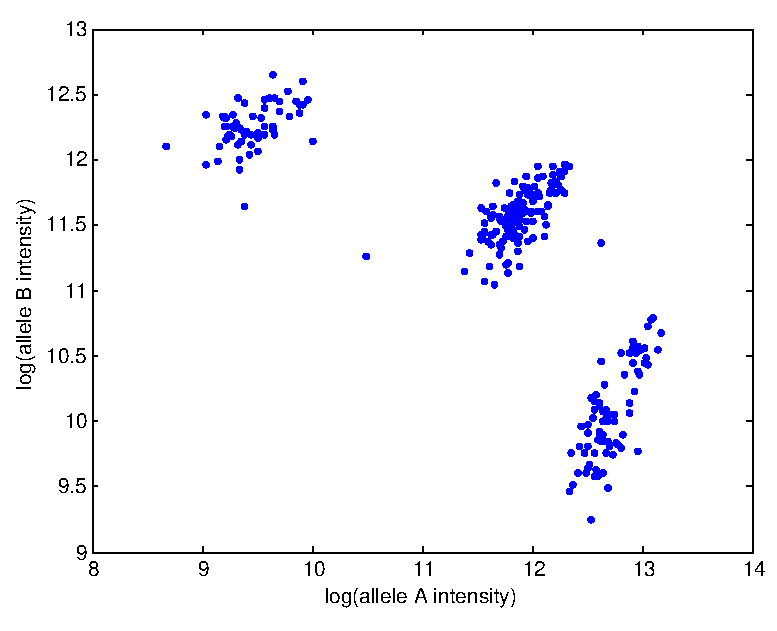
\includegraphics[scale=0.5]{method_figs/defined_cluster.pdf}
        \label{fig:defined_cluster}
    }
    \subfloat[SNP with sparse BB genotype cluster] {
        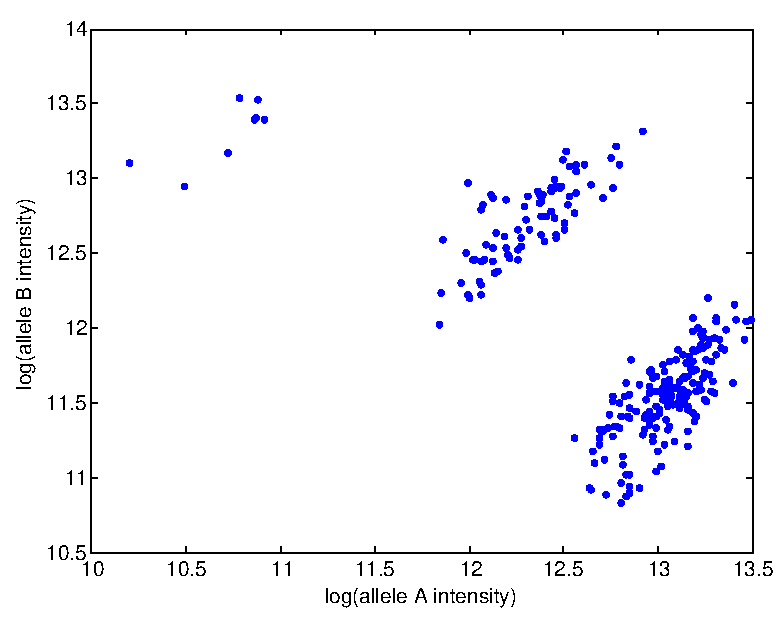
\includegraphics[scale=0.5]{method_figs/sparse_cluster.pdf}
        \label{fig:sparse_cluster}
    }
    \caption{SNPs with moderate MAF have well defined genotype clusters,
             whereas SNPs with lower MAF may have sparse genotype clusters.}
    \label{fig:defined_sparse_cluster}
\end{figure}

% missing genotype aa cluster
\subsubsection{Missing genotype AA or BB cluster}

\par
If the genotype $AA$ cluster of a SNP has less than 5 reference calls, SoCal
first finds the ellipsoids for genotype $AB$ and $BB$ clusters, and then
estimates that for genotype $AA$ cluster through simple geometric
transformations.

\par
Let $\mathcal{E}_{AB}=
\{x \in \mathbbm{R}^{n}|(x-c_{AB})^TE_{AB}(x-c_{AB}) \leqslant 1\}$
and $\mathcal{E}_{BB}=
\{x \in \mathbbm{R}^{n}|(x-c_{BB})^TE_{BB}(x-c_{BB}) \leqslant 1\}$
be the ellipsoids obtained for genotype $AB$ and $BB$ clusters,
and $n_{AB}$, $n_{BB}$ the unit vectors pointing in the direction of
the major axis of the corresponding ellipsoid.
SoCal estimates the center of $\mathcal{E}_{AA}$, the ellipsoid for genotype
$AA$ cluster, by reflecting $c_{BB}$, the center of $\mathcal{E}_{BB}$, across
the major axis of $\mathcal{E}_{AB}$.
To estimate the orientation of $\mathcal{E}_{AA}$, SoCal first determines the
angle between $n_{AB}$ and $n_{BB}$, and then applies a rotation matrix of
that angle on $E_{AB}$.

\par
Formally, let $\mathcal{E}_{AA}=
\{x \in \mathbbm{R}^{n}|(x-c_{AA})^TE_{AA}(x-c_{AA}) \leqslant 1\}$ be the
estimated ellipsoid for genotype $AA$ cluster, and $\alpha$ the angle between
$n_{AB}$ and $n_{BB}$, then
$c_{AA}=-c_{BB}+2c_{AB}+2n_{AB}((c_{BB}-c_{AB})^{T}n_{AB})$, and
$E_{AA}=R^{T}E_{AB}R$, where $R$ is a rotation matrix of angle $\alpha$.

\par
If genotype $BB$ cluster is missing, the center and orientation of the
ellipsoid for that cluster is estimated in a similar way.
Formally, let $\mathcal{E}_{BB}=
\{x \in \mathbbm{R}^{n}|(x-c_{BB})^TE_{BB}(x-c_{BB}) \leqslant 1\}$ be the
estimated ellipsoid for genotype $BB$ cluster, and $\alpha$ the angle between
$n_{AB}$ and $n_{AA}$, then
$c_{BB}=-c_{AA}+2c_{AB}+2n_{AB}((c_{AA}-c_{AB})^{T}n_{AB})$, and
$E_{BB}=R^{T}E_{AB}R$, where $R$ is a rotation matrix of angle $-\alpha$.

% missing genotype ab cluster
\subsubsection{Missing genotype AB cluster}

Although SNPs with genotype $AB$ cluster missing were not observed in HapMap
reference genotype calls, for completeness, for these SNPs SoCal first
obtains, $\mathcal{E}_{AA}$ and $\mathcal{E}_{BB}$,
the ellipsoids for genotype $AA$ and $BB$ cluster, and then estimates the
center of $\mathcal{E}_{AB}$, the ellipsoid for the missing cluster, using
the mid-point between the centers of $\mathcal{E}_{AA}$ and $\mathcal{E}_{BB}$.
The orientation of $\mathcal{E}_{AB}$ is obtained by applying a rotation
to the ellipsoid with the minimum volume among $\mathcal{E}_{AA}$ and
$\mathcal{E}_{BB}$.

\par
Formally, let $\mathcal{E}_{AB}=
\{x \in \mathbbm{R}^{n}|(x-c_{AB})^TE_{AB}(x-c_{AB}) \leqslant 1\}$ be the
estimated ellipsoid for genotype $AB$ cluster, and $\alpha$ the angle between
$n_{AA}$ and $n_{BB}$, then
$c_{AB}=(c_{AA}+c_{BB})/2$, and
$E_{AB}=R^{T}\hat{E}R$, where $\hat{E}$ is the matrix of the ellipsoid
with the minimum volumne among $\mathcal{E}_{AA}$ and $\mathcal{E}_{BB}$, and
$R$ a rotation matrix of angle $\pm\alpha/2$.
The sign of the angle of rotation is dependent on the choise of ellipsoid on
which rotation is applied---positive for $\mathcal{E}_{AA}$ and negative
for $\mathcal{E}_{BB}$.

% genotype calling and outlier detection
\subsection{Genotype calling}

\par
After the ellipsoidal decision regions,
$\mathcal{E}_{g}=
\{x \in \mathbbm{R}^{n} | (x-c_g)^TE_g(x-c_g) \leqslant 1\},
\forall g\in\{AA,AB,BB\}$ of a SNP are obtained, SoCal uses them to classify
samples with unknown genotypes using minimum distance classification.

\par
If a sample has allele intensity $\theta_A$ and $\theta_B$ at SNP $n$,
SoCal first computes
$D_g=\sqrt{(x-c_g)^TE_g(x-c_g)}$,
where $x=(log(\theta_A), log(\theta_B))$, for each $g\in\{AA,AB,BB\}$.
SoCal then calls the genotype, $\mathcal{G}$, of that sample at SNP $n$
as the genotype having the minimum $D_g$, that is,
$\mathcal{G}=\operatorname*{arg\,min}_{g\in \{AA,AB,BB\}}D_g$.
SoCal defines $\lambda=1-D_{\mathcal{G}}/(D_{AA}+D_{AB}+D_{BB})$ to quantify
the confidence of each genotype call. 
%-----------------------------------------------------------------------------










%-----------------------------------------------------------------------------
% data

\section{Data}
TODO: Write data section
filter out monomorphic snps

%-----------------------------------------------------------------------------










%-----------------------------------------------------------------------------
% result

\section{Result}

% result for comparing socal with hapmap calls
\subsection{Comparison with HapMap reference calls}

% 100% call rate result
\begin{table}[H]
\centering
\begin{tabular}{l*{5}{r}r}
    \hline
    HapMap/SoCal  & AA       & AB      & BB      & No Call \\ \hline
    AA            & 360,289  & 2,282   & 1,058   & 0  \\
    AB            & 2,667    & 341,012 & 2,257   & 0  \\
    BB            & 851      & 2,347   & 368,556 & 0  \\ \hline
\end{tabular}
\caption{At a call rate of 100\%, SoCal achieved 98.94\% concordance rate
in the leave-one-out cross-validation with HapMap reference calls.}
\label{table:cmp_hapmap_socal}
\end{table}

% 95% call rate result
\begin{table}[H]
\centering
\begin{tabular}{l*{5}{r}r}
    \hline
    HapMap/SoCal  & AA       & AB      & BB      & No Call \\ \hline
    AA            & 348,221  & 390     & 298     & 14,720  \\
    AB            & 710      & 319,394 & 775     & 25,057  \\
    BB            & 410      & 427     & 357,627 & 13,290  \\ \hline
\end{tabular}
\caption{At a call rate of 95\%, SoCal achieved 99.71\% concordance rate
in the leave-one-out cross-validation with HapMap reference calls.}
\label{table:cmp_hapmap_socal}
\end{table}

% accuracy as function of call rate
\begin{figure}[H]
\centering
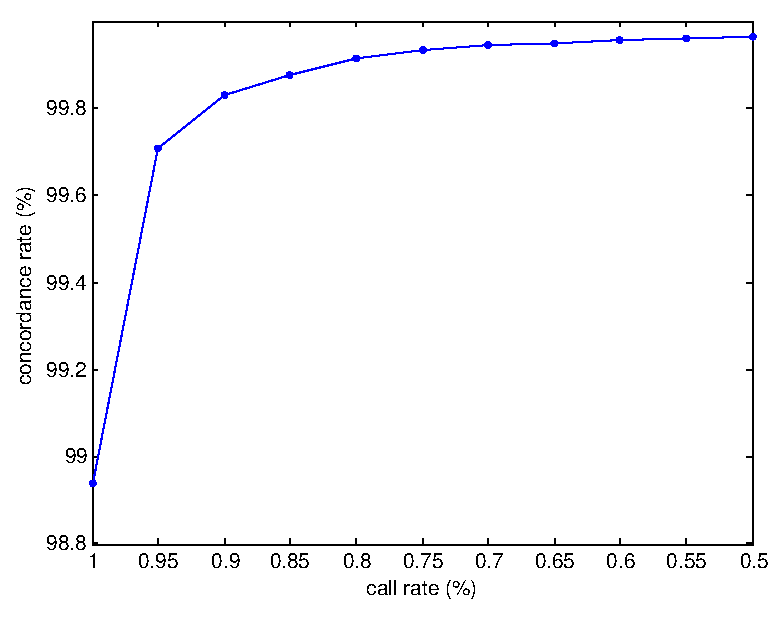
\includegraphics[scale=0.75]
{result_figs/cmp_socal_hapmap/cmp_socal_hapmap_cr_vs_acc.pdf}
\caption{Concordance rate of SoCal in the leave-one-out cross-validation with
HapMap reference calls as a function of call rate.}
\label{fig:result_sh_crvacc}
\end{figure}


\subsection{Comparison with CRLMM calls}
TODO: Compare with CRLMM
concordance rate
call rate

\subsection{Simulating error calls}
TODO: Simulate error calls - assign ab to aa, ab to bb, aa to ab, bb to ab
aa to bb, bb to aa
concordance rate
call rate
before
after
select good snps
compare with rlmm - fitting gaussian

%-----------------------------------------------------------------------------











%-----------------------------------------------------------------------------
% discussion

\section{Discussion}
TODO: Write discussion section

%-----------------------------------------------------------------------------









%-----------------------------------------------------------------------------
% references

\begin{thebibliography}{9}
\bibitem{rho2010}
Rho, S. W., Abell, G. C., Kim, K., Nam, Y., \& Bae, J. (2010).
Comparing microarrays and next-generation sequencing technologies for microbial
ecology research. Trends in Biotechnology, 28, 291-299.
\bibitem{norlen2008}
Norl\'{e}n, H., Pettersson, E., Ahmadian, A., Lundeberg, J., \& Sundberg, R.
(2008). Classification of SNP genotypes by a Gaussian mixture model in
competitive enzymatic assays.
Mathematical Statistics Stockholm University Research Report, 3, 1-26.
\bibitem{lin2008}
Lin, Y., Tseng, G. C., Cheong, S. Y., Bean, L. J., Sherman, S. L., \&
Feingold, E. (2008). Smarter clustering methods for SNP genotype calling.
Bioinformatics, 24, 2665-2671.
\bibitem{wu1983}
Wu, C. F. (1983). On the Convergence Properties of the EM Algorithm.
The Annals of Statistics, 11, 95-103.
\bibitem{rabbee2005}
Rabbee, N., \& Speed, T. P. (2005).
A genotype calling algorithm for affymetrix SNP arrays.
Bioinformatics, 22, 7-12.
\bibitem{zhou2014}
Zhou, X., \& Stephens, M. (2014).
Efficient multivariate linear mixed model algorithms for genome-wide
association studies.
Nature Methods, 11, 407-409.
\bibitem{glineur1998}
Glineur F. (1998). Pattern separation via ellipsoids and conic programming.
(MS Thesis). Faculté Polytechnique de Mons, Mons, Belgium.
\end{thebibliography}

%-----------------------------------------------------------------------------

\end{document}
